\chapter{Spule und Transformator}
\label{v:16}

In diesem Versuch lernen Sie einige Eigenschaften von Spulen und Transformatoren kennen.

%------------------------------------------------
\section{Stichworte}
%------------------------------------------------

Lorentzkraft; Induktionsgesetz; magnetischer Fluss; Selbstinduktion; Effektivwerte für $U$ und $I$; Wechselstromwiderstände; unbelasteter und belasteter Transformator; Spannungsübersetzungsverhältnis.
%
%------------------------------------------------
\section{Literatur}
%------------------------------------------------

Gehrtsen, Kapitel 7.2.3, 7.3.2/5, 7.5.8
%
%------------------------------------------------
\section{Anwendungsbeispiele}
%------------------------------------------------

Unser heutiges Leben wird so sehr von elektrischen Geräten bestimmt, dass man von der ''Elektrozeit'' sprechen könnte. Elektrischer Strom wird meist in Generatoren hergestellt, die mechanische Drehbewegungen (Wasserturbinen, Dampfturbinen, Windräder) ausnutzen, um eine Spule im Magnetfeld zu drehen. Dabei wirkt das Induktionsgesetz. Es bedeutet in Worten, dass jede zeitliche Änderung des magnetischen Flusses eine elektrische Spannung induziert. Es zeigt den Zusammenhang zwischen dem elektrischen und dem magnetischen Feld, wenn beide sich zeitlich verändern und ist von größter Bedeutung in der Elektrotechnik.\\
Die zweite wichtige Anwendung des Induktionsgesetzes ist der Transformator. Er spielt bei der Stromversorgung eine wichtige Rolle, da durch die Hochspannungstransformation (\unit{110}{\kilo}{\volt} bis \unit{380}{\kilo}{\volt}) die Stromstärken für den Transport verringert werden können und somit nach $P = I^2 R$ geringere Verlustleistungen auftreten. ''Tausende'' kleiner Transformatoren umgeben uns überall, um die Wechselspannung von \unit{220}{\volt} aus dem Netz auf die 6 - 12\,V Gleichspannung herunter zu transformieren (bei zusätzlicher Gleichrichtung), die von unseren elektronischen Helfern benötigt werden. Diese kleinen Trafos sind immer warm oder heiß und verbrauchen ständig elektrische Leistung, wenn sie mit dem Netz verbunden sind.\\
Im Versuch wird ein einfacher Transformator untersucht. Es wird versucht, den Begriff der Phase bei Wechselspannungen näher zu bringen.

%------------------------------------------------
\section{Theoretischer Hintergrund}
%------------------------------------------------


\subsection{Transformator}

Ein Transformator betseht aus zwei Spulen, die so angeordnet sind, daß das bei Stromfluß in einer Spule entstehende magnetische Feld die Windungsfläche der anderen Spule durchsetzt und umgekehrt. Jede zeitliche Änderung des Stroms in einer Spule induziert in der anderen - und natürlich in sich selbst - eine Spannung.\\
Man kann daher Leistung von einem mit der Primärspule verbundenen Stromkreis auf einen mit der Sekundärspule verbundenen Kreis übertragen, ohne daß beide Kreise galvanisch (d.h. leitend) miteinander verbunden sind. Häufig wickelt man beide Spulen auf einen (z.B. ringförmig geschlossenen) Eisenkern, um zu erreichen, daß alle magnetischen Feldlinien die Windungsflächen beider Spulen durchsetzen. Die jeweiligen magnetischen Flüße $\Phi_{m,i}$ (i=1,2) und damit die induzierten Spannungen verhalten sich wie die Windungszahlen der Spulen. \\

\noindent
\begin{minipage}{0.6\textwidth}
In der Abbildung rechts sind die beiden Spulen (Windungszahlen $N_1$ und $N_2$) auf ein geschlossenes Eisenjoch gewickelt. An die Primärspule legen wir die Wechselspannung $U_1$ an. Die Sekundärspule schliessen wir mit einer Impedanz Z ab. In der Primärspule fließt ein sinusförmiger, gegen $U_1$ phasenverschobener Strom $I_1$, der wiederum einen zeitlich veränderlichen magnetischen Fluß $\Phi_{m,1}$ hervorruft. Der alternierende magnetische Fluß induziert in der Sekundärspule eine Wechselspannung
\begin{equation}
U_{ind} = -L_1\frac{dI_1}{dt} = -N_1\frac{d\Phi_{m,1}}{dt}\; .
\end{equation}
\end{minipage}
%
\begin{minipage}{0.4\textwidth}
	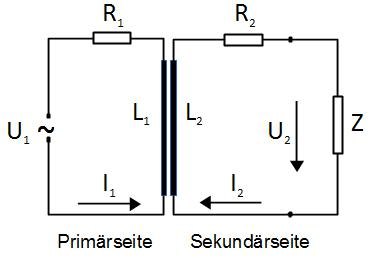
\includegraphics[width=\textwidth]{Abbildungen/Trafo1.jpg}
	\label{fig:Trafo1}
\end{minipage}
%

\noindent
Diese ist nach den Kirchhoff'schen Regeln der von außen angelegten Spannung entgegengesetzt gleich. Wenn der gesamte in der Primärspule erzeugte magnetische Fluß auch durch die Sekundärspule $L_2$ geht, wird dort eine Spannung
\begin{equation}
U_2 = -N_2\frac{d\Phi_{m,1}}{dt}
\end{equation}
induziert. Durch Z und die Spule fließt daraufhin ein Wechselstrom $I_2$. Auch dieser trägt zur Magnetisierung des Kerns bei und veranlaßt eine Rückwirkung des Sekundärkreises auf den Primärkreis (Gegeninduktion).\\
An jeder Spule liegen daher zwei induzierte Spannungen, die den zeitlichen Ableitungen der magnetischen Teilflüsse und damit den zeitlichen Ableitungen der sie erregenden Ströme $I_1$ bzw. $I_2$ proportional sind. Mit den in der Abbildung angegebenen Richtungen, den Induktivitäten von Primär- und Sekundärspule $L_1$und $L_2$, der Gegeninduktivität (mutual inductivity) der beiden Spulen $M$ und den zu den Spulen in Reihe geschalteten Widerständen $R_1$, $R_2$ erhält man die Transformatorgleichungen
\begin{align*}
U_1 & = (i\omega L_1 + R_1) I_1 + i\omega M I_2 &\\
U_2 & = i\omega M I_1 + (i\omega L_2 + R_2) I_2 \; .
\end{align*}

Die Induktivitäten $L_1$, $L_2$ sind proportional zu den Quadraten der Windungszahlen $N_1$, $N_2$ von Primär- und Sekundärspule. Für die Gegeninduktivität gilt $M\propto N_1N_2$. Wenn der gesamte magnetische Fluß beide Spulen durchsetzt gilt weiterhin: $M^2 = L_1L_2$\; . Im Folgenden wollen wir einen verlustlosen Transformator betrachten: $R_1 = R_2 = 0$\; .\\
Für einen \textit{unbelasteten Transformator} ($R = \infty$) findet man dann für die Spannungsübersetzung:
\begin{equation} \label{eq:Spannungsuebersetzung}
\frac{U_2}{U_1} = \frac{M}{L_1} = \frac{N_2}{N_1}\; .
\end{equation}

\noindent
Für die Stromübersetzung im Kurzschlußfall findet man:
\begin{equation} \label{eq:Stromuebersetzung}
\frac{I_2}{I_1} = \frac{M}{L_2} = \frac{N_1}{N_2}
\end{equation}
%------------------------------------------------
\section{Fragen zur Vorbereitung}
%------------------------------------------------

\begin{enumerate}
	%
	\item Was ist eine Wechselspannung/ein Wechselstrom? Wie kann man sie/ihn mathematisch beschreiben (Beispiel)?
	%
	\item Was versteht man unter einer Effektivspannung/ einem Effektivstrom? Wie lautet der entsprechende Zusammenhang für eine sinusförmige Wechselspannung?
	%
	\item Was versteht man unter elektrischer Leistung? Was gilt für die mittlere elektrische Leistung in einem Wechselstromkreis? (Stichwort: Phasenverschiebung zwischen Strom und Spannung)
	%
	\item Wie lautet der Zusammenhang zwischen Strom und Spannung für einen ohmschen Widerstand in einem Wechselstromkreis?
	%
	\item Wie lautet der Zusammenhang zwischen Strom und Spannung für den kapazitiven Widerstand eines idealen Kondensators in einem Wechselstromkreis?
	%
	\item Wie lautet der Zusammenhang zwischen Strom und Spannung für den induktiven Widerstand einer idealen Spule in einem Wechselstromkreis?
	%
%	\item Wie lautet der Zusammenhang für den Gesamtwiderstand (Impedanz) einer Reihenschaltung von ohmschen, kapazitiven und induktiven Widerstand in einem Wechselstromkreis?
	%
%	\item Was haben das Magnetfeld eines Stabmagneten und das einer Spule gemeinsam? Wie sieht der Verlauf der Feldlinien aus?
	%
	\item Wie verlaufen die Magnetfeldlinien im Inneren einer langen Spule? Welcher Zusammenhang gilt zwischen magnetischer Flussdichte B und Stromstärke I (keine detaillierte Formel, nur proportional, quadratisch, reziprok o.ä.)?
	%
	\item Was ist die Lorentzkraft? Wie ist sie definiert?
	%
	\item Was besagt das Induktionsgesetz? Welche Bedeutung hat das Minuszeichen (Stichwort: Lenzsche Regel)?
	%
	\item Was ist ein Transformator und wozu dient er? Wie ist er aufgebaut? Welche Aufgabe hat der Eisenkern?
	%
	\item Was versteht man unter einem unbelasteten Transformator? Was versteht man unter einem belasteten Transformator? (Hilfe: Schaltskizze)
	%
%	\item Wie leitet sich das Spannungsübersetzungsverhältnis $\frac{U_1}{U_2}=\frac{N_1}{N_2}$ bzw. das Stromübersetzungsverhältnis $\frac{N_1}{N_2}=\frac{I_2}{I_1}$ beim Transformator ab ?
 %
\end{enumerate}

%------------------------------------------------
\section{Durchführung} 
%------------------------------------------------

\begin{enumerate}
	%
	\item \label{VT1}
	%\textit{Der Folgende Versuchsteil wird durch den Assistenten durchgeführt:}\\
		\textbf{Phasenverschiebung an einer Spule:}\\
		Man schließe den Schiebewiderstand in Reihe mit der Primärspule (Spule 1 = Sp1) des Transformators und verbinde sie direkt mit dem Ausgang des Netzgerätes. Man stelle die Spannung an der Spule und die Spannung am Ausgang des 
		Netzgerätes auf dem Oszilloskop dar.\\
		
		\etodo{Schaltskizzen in tikz neu zeichnen!}
		\begin{minipage}{0.7\textwidth}
			\centering
				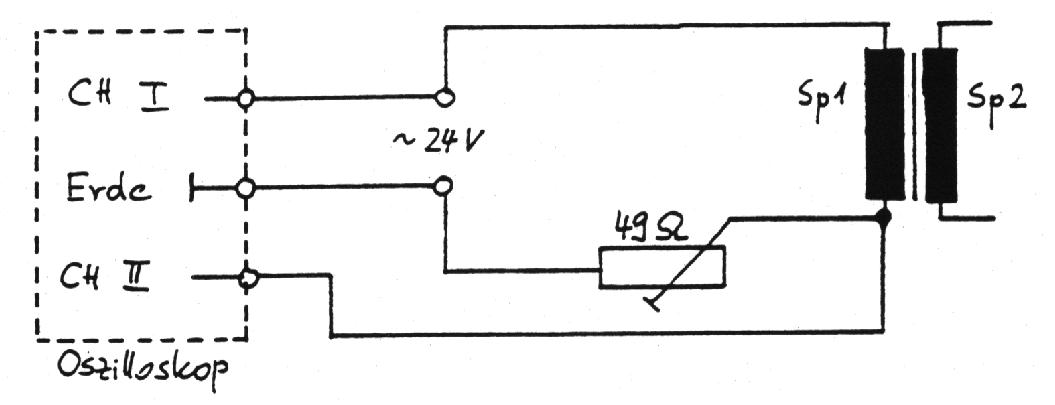
\includegraphics[width=0.90\textwidth]{Abbildungen/Bild31.jpg}
			\label{fig:Bild31}
		\end{minipage}
		%
		\begin{minipage}{0.3\textwidth}
			\centering
				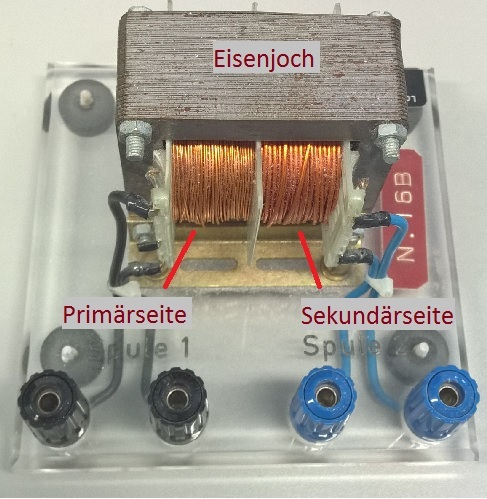
\includegraphics[width=0.90\textwidth]{Abbildungen/Trafo.jpg}
			\label{fig:Trafo_Foto}
		\end{minipage}
		
		Dazu verbinde man Kanal 1 (CH I) mit einem Pol des Netzgeräts, den anderen Pol mit der Erde des Oszilloskops. Kanal 2 (CH II) wird mit der Spule gemäss Schaltbild verbunden. Das Wechselspannungs-Netzgerät wird auf 25\% 
		der Leistung reduziert. Man messe (qualitativ) die Phasenverschiebung zwischen den beiden Signalen! Beträgt die Phasenverschiebung 0°, 90° oder liegt sie dazwischen?
	%
	\item \textbf{Unbelasteter Transformator:}\\ 
		Man benutze Spule 1 als Primärspule und Spule 2 als Sekundärspule.\\
		\begin{minipage}{0.55\textwidth}
			Messen Sie mit dem Oszilloskop die Sekundärspannung $U_2$ in Abhängigkeit der Primärspannung $U_1$. Variieren Sie dazu $U_1$ in Schritten von 3\,V im Bereich $0\leq U_1\leq 24$\,V.\\
			\textit{Hinweis: Die Spannungsangaben in der Zeichnung stellen die empfohlenen Messbereiche der Voltmeter dar.}
		\end{minipage}
		%
		\begin{minipage}{0.45\textwidth}
			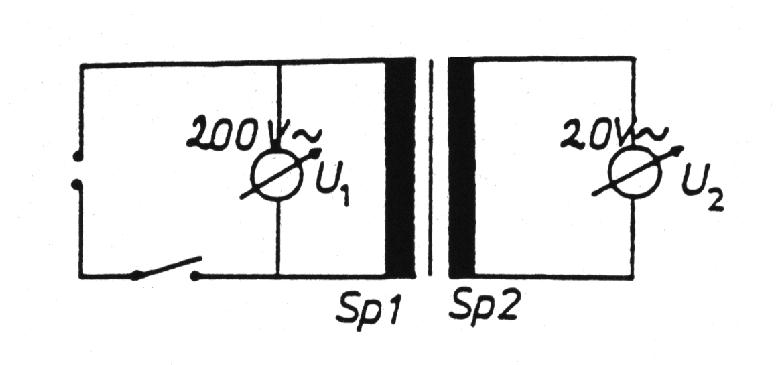
\includegraphics[width=\textwidth]{Abbildungen/BILD20.jpg}
			\label{fig:Bild20}
		\end{minipage}
	%
	\item \textbf{Belasteter Transformator:}\\
	Bevor Sie mit diesem Versuchsteil beginnen, lesen Sie bitte die gesamte Anleitung, inklusive des unten stehenden Kastens, aufmerksam durch. Bei diesem Versuchsteil können Sie ansonsten gehörigen Schaden an den Geräten anrichten!\\
	
	\noindent
	Legen Sie an die Primärspule 1 eine Spannung $U_{eff}$\,=\,20\,V und bauen Sie in den Sekundärkreis einen ohmschen Widerstand ein.\\
		\begin{minipage}{0.55\textwidth}
			Messen Sie den Strom auf der Primärseite $I_1$ in Abhängigkeit des Stroms auf der Sekundärseite $I_2$. Variieren Sie dazu $I_2$ in Schritten von 0,2\,A im Bereich $0\leq I_2\leq 2$\,A.\\
		\end{minipage}
		%
		\begin{minipage}{0.45\textwidth}
			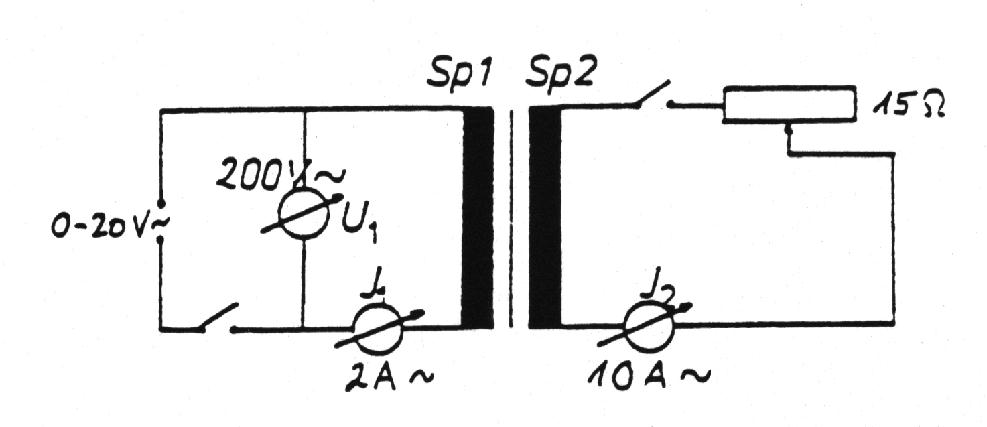
\includegraphics[width=\textwidth]{Abbildungen/BILD22.jpg}
			\label{fig:Bild22}
		\end{minipage}
		
	\begin{hint}
	\begin{enumerate}[label={\roman*}.]
		%
		\item Achten Sie darauf, dass die Spannung im Primärkreis während des gesamten Versuchs bei konstant $U_1$\,=\,20\,V liegt! Regeln Sie ggf. nach!
		%
		\item Vorsicht bei der Regulierung der Stromstärke $I_2$ durch Verschieben des regelbaren Widerstandes. Die Stromstärke ändert sich nicht linear mit der Verschiebung des Widerstandes. D.h. bei kleinen Stromstärken $I_2$ 
			führen kleine Verschiebungen zu kleinen Änderungen von $I_2$, bei großen Stromstärken führen kleine Verschiebungen des Widerstandes zu großen Änderungen der Stromstärke $I_2$.\\
			\textbf{Messgeräte nicht überlasten! Wenn die Strommessung plötzlich nicht mehr funktioniert, dann ist die Sicherung des Messgeräts durchgebrannt. Bitte den Tutoren Bescheid geben!}
		%
	\end{enumerate}
	\end{hint}
	%
	\etutorhint{Trotz des Hinweises oben werden die Studierenden es schaffen, ein paar Sicherungen zu schrotten. Bitte die betroffenen Multimeter einfach auf dem Tisch neben dem Messgeräteschrank abstellen, dann reparieren wir die.}
\end{enumerate}

%------------------------------------------------
\section{Auswertung} 
%------------------------------------------------
\etodo{Musterauswertung}

\begin{hint}
	Bitte fertigen Sie die Graphen in der folgenden Auswertung per Hand auf Millimeterpapier an.
\end{hint}

\begin{enumerate}
%
\item Erklären Sie kurz den Begriff ''Phasenverschiebung'' am Beispiel von Versuchsteil \ref{VT1}.. Warum ist die dort beobachtete Phasenverschiebung kleiner als 90\degree?
%
\item Stellen Sie die Messreihe $U_2\,=\,f(U_1)$ graphisch dar! Bestimmen Sie aus der Steigung der Auftragung das Spannungsübersetzungsverhältnis $U_2/U_1$. Beachten Sie dabei, dass die Steigung auch eine Unsicherheit hat!

	\noindent
	\textbf{Bemerkung:} Es kann vorkommen, dass ''so gut'' gemessen wurde, dass alle Messwerte auf einer Geraden liegen, so dass sich keine ''sinnvollen'' Fehlergeraden einzeichnen lassen. Bestimmen Sie in diesem Fall (und nur in
	diesem Fall!!!) das Spannungsübersetzungsverhältnis als Mittelwert mit Standardabweichung aus den Einzelmessungen des Spannungsübersetzungsverhältnisses $U_2/U_1$! D.h. berechnen Sie die einzelnen Verhältnisse und dann den Mittelwert daraus. \\
	Eine korrekte Fehlerrechnung wird für den weiteren Teil der Auswertung benötigt!
%
\item Stellen Sie die Messreihe $I_1\,=\,f(I_2)$ graphisch dar! Bestimmen Sie aus der Steigung der Auftragung das Stromübersetzungsverhältnis $I_1/I_2$ (mit Fehler)!

	\noindent
	\textbf{Bemerkung:} Obwohl man annimmt, dass $I_1/I_2\, =\,N_2/N_1$ gilt, ergibt die graphische Auftragung keine Gerade. Das liegt daran, dass bei der Herleitung des o.g. Zusammenhangs stark idealisiert wurde!
%
\item Die Windungszahl der Sekundärspule beträgt $N_2\,=\,72$. Bestimmen Sie anhand der Beziehungen $U_2/U_1\,=\,N_2/N_1$ für den unbelasteten Transformator und $I_1/I_2\,=\,N_2/N_1$ für den belasteten Transformator jeweils die Windungszahl $N_1$ der Primärspule inklusive ihres Fehlers.
%
\item Berechnen Sie anhand der beiden Einzelergebnisse für $N_1$ den gewichteten Mittelwert von $N_1$ (mit Fehler des gewichteten Mittelwerts)!
%
\end{enumerate}